\section{Question 2}
    \subsection{Tìm vị trí các máy bay trong hình bằng phương pháp genral hough transform tự lập trình}
        \subsubsection{Các bước thực hiện}
            \begin{itemize}
                \item Tạo các Template của các máy bay trong hình.
                \begin{figure}[H]
                    \centering
                    
\includegraphics[width=0.6\textwidth]{pictures/chapter2/c02_p01_Template.png}
                    \caption{Các Template của các máy bay trong hình}
                \end{figure}
                \item Load Template và Scene:
                \begin{lstlisting}
tpl = cv2.imread(TEMPLATE_PATH, cv2.IMREAD_GRAYSCALE)
scene = cv2.imread(SCENE_PATH)
scene_gray = cv2.cvtColor(scene, cv2.COLOR_BGR2GRAY)
                \end{lstlisting}
                \item Xây R-table - với GHT ta lưu cho mỗi hướng biên (edge orientation bin) một hoặc nhiều vector chỉ từ điểm biên tới tham chiếu (center) của template. Khi dò trong ảnh scene, từ mỗi điểm biên cộng vector này sẽ ước lượng vị trí center ứng viên.
                \begin{lstlisting}
def build_rtable(template_gray):
    _, bin_img = cv2.threshold(template_gray, 0, 255, cv2.THRESH_BINARY + cv2.THRESH_OTSU)
    edges = cv2.Canny(bin_img, CANNY_LOW, CANNY_HIGH)

    gx = cv2.Sobel(template_gray, cv2.CV_32F, 1, 0, ksize=3)
    gy = cv2.Sobel(template_gray, cv2.CV_32F, 0, 1, ksize=3)
    
    ys, xs = np.where(bin_img > 0)
    if len(xs) == 0:
        raise ValueError("Template was empty after thresholding.")
    cx, cy = xs.mean(), ys.mean()

    ys_e, xs_e = np.where(edges > 0)
    
    # Vectorized: Compute orientations for all edge points
    theta = np.arctan2(gy[ys_e, xs_e], gx[ys_e, xs_e])
    theta = np.degrees(theta) % 360.0
    bin_ang = (theta // ANGLE_BIN).astype(int) * ANGLE_BIN

    rx = cx - xs_e
    ry = cy - ys_e
    
    # Create R-table bins
    n_bins = 360 // ANGLE_BIN
    rtable_bins = np.arange(0, 360, ANGLE_BIN)
    
    # Build R-table index
    rtable_idx = {}
    for b in rtable_bins:
        mask = bin_ang == b
        if np.any(mask):
            rtable_idx[b] = np.where(mask)[0]
    
    # Stack r vectors
    r_vectors = np.column_stack([rx, ry])  # shape: (N_edges, 2)
    
    return rtable_idx, r_vectors, (cx, cy)
                \end{lstlisting}
                \item Thực hiện voting cho tất cả rotation và scale, tạo accumulator 4D: (H, W, n\_scales, n\_rotations). Mỗi vote tăng 1 tại vị trí center (x,y) tương ứng scale và rotation.
                \begin{lstlisting}
def vote_with_rot_scale_vectorized(scene_gray, rtable_idx, r_vectors):
    edges = cv2.Canny(scene_gray, CANNY_LOW, CANNY_HIGH)
    gx = cv2.Sobel(scene_gray, cv2.CV_32F, 1, 0)
    gy = cv2.Sobel(scene_gray, cv2.CV_32F, 0, 1)

    H, W = scene_gray.shape
    n_rots = len(ROTATIONS)
    n_scales = len(SCALES)

    # Create 4D accumulator: [H, W, n_scales, n_rots]
    acc_4d = np.zeros((H, W, n_scales, n_rots), dtype=np.int32)

    ys_scene, xs_scene = np.where(edges > 0)
    n_scene = len(xs_scene)
    
    if n_scene == 0:
        return acc_4d

    # Scene angles for all edge pixels
    theta_scene = np.arctan2(gy[ys_scene, xs_scene], gx[ys_scene, xs_scene])
    theta_scene = np.degrees(theta_scene) % 360.0  # shape: (n_scene,)
    
    print(f"Processing {n_scene} scene edges...")

    # Strategy: Process in batches of (rotation, scale) combinations
    
    for rot_idx in range(n_rots):
        phi = ROTATIONS[rot_idx]
        cos_phi = ROT_COS[rot_idx]
        sin_phi = ROT_SIN[rot_idx]
        
        # Template angles corresponding to scene angles when rotated by phi
        theta_tpl = (theta_scene - phi) % 360.0  # (n_scene,)
        bin_tpl = ((theta_tpl // ANGLE_BIN).astype(int) * ANGLE_BIN) % 360
        
        # Rotate ALL r_vectors at once
        # r_rotated shape: (n_template_edges, 2)
        r_rotated = np.empty_like(r_vectors)
        r_rotated[:, 0] = r_vectors[:, 0] * cos_phi - r_vectors[:, 1] * sin_phi
        r_rotated[:, 1] = r_vectors[:, 0] * sin_phi + r_vectors[:, 1] * cos_phi
        
        for scale_idx, scale in enumerate(SCALES):
            # Scale ALL rotated vectors
            r_scaled = r_rotated * scale  # (n_template_edges, 2)
            
            # For each bin, vote ALL combinations at once
            for bin_val, template_indices in rtable_idx.items():
                # Get scene edges belonging to this bin
                scene_mask = bin_tpl == bin_val
                scene_indices = np.where(scene_mask)[0]
                
                if len(scene_indices) == 0:
                    continue
                
                # Get scene edge coordinates
                xs_s = xs_scene[scene_indices]  # (n_s,)
                ys_s = ys_scene[scene_indices]  # (n_s,)
                
                # Get r vectors from template for this bin
                r_bin = r_scaled[template_indices]  # (n_t, 2)
                
                # VECTORIZED OUTER SUM:
                # Each scene edge (xs_s[i], ys_s[i]) + each r_bin[j]
                # Create mesh: (n_s, n_t, 2)
                xs_mesh = xs_s[:, None] + r_bin[:, 0][None, :]  # (n_s, n_t)
                ys_mesh = ys_s[:, None] + r_bin[:, 1][None, :]  # (n_s, n_t)
                
                # Round and flatten
                xi = np.round(xs_mesh).astype(int).ravel()
                yi = np.round(ys_mesh).astype(int).ravel()
                
                # Filter valid
                valid = (xi >= 0) & (xi < W) & (yi >= 0) & (yi < H)
                xi = xi[valid]
                yi = yi[valid]
                
                # Vote using np.add.at (atomic add)
                np.add.at(acc_4d, (yi, xi, scale_idx, rot_idx), 1)
    
    return acc_4d
                \end{lstlisting}
                \item Tìm vị trí đỉnh trên accumulator (peak detection) theo NMS.
                \begin{lstlisting}
def find_peaks_vectorized(acc_4d):
    max_val = acc_4d.max()
    if max_val == 0:
        return []
    
    # Normalize
    acc_norm = acc_4d.astype(np.float32) / max_val
    
    # Apply threshold
    acc_thresh = acc_norm * (acc_norm >= ACC_REL_THRESH)
    
    # Non-maximum suppression in 4D
    # Apply local maximum filter
    footprint = np.ones((5, 5, 1, 1))  # spatial NMS only
    local_max = maximum_filter(acc_thresh, footprint=footprint, mode='constant')
    
    # Peaks are where values equal local max
    peaks_mask = (acc_thresh == local_max) & (acc_thresh > 0)
    
    # Get peak coordinates
    coords = np.argwhere(peaks_mask)  # (N_peaks, 4)
    scores = acc_thresh[peaks_mask]
    
    # Sort theo score
    sort_idx = np.argsort(-scores)[:MAX_PEAKS]
    
    peaks = []
    for idx in sort_idx:
        y, x, scale_idx, rot_idx = coords[idx]
        score = scores[idx]
        peaks.append((int(x), int(y), float(score), 
                     float(SCALES[scale_idx]), int(ROTATIONS[rot_idx])))
    
    return peaks                
                \end{lstlisting}
                \item Tạo bản sao của ảnh gốc scene, sau đó vẽ lên đó vị trí các peak mà GHT tìm được—nghĩa là những chỗ được dự đoán là tâm (center) của template.
                \begin{lstlisting}
vis = scene.copy()
    for (x, y, s, scale, rot) in peaks:
        cv2.circle(vis, (int(x), int(y)), 20, (0, 255, 0), 2)
        cv2.putText(vis, f"{s:.2f} s={scale:.2f} r={rot}deg", (int(x)-40, int(y)-25),
                    cv2.FONT_HERSHEY_SIMPLEX, 0.5, (0,255,0), 2)

    cv2.imwrite(OUT_PATH, vis)
    print("Saved to:", OUT_PATH)
                \end{lstlisting}
            \end{itemize}
        \subsubsection{Kết quả thu được}
            \begin{itemize}
                \item Với template 1:
                \begin{figure}[H]
                    \centering
                    
\includegraphics[width=0.3\textwidth]{pictures/chapter2/c02_p02_template_1.png}
                    \caption{Template 1}
                \end{figure}
                Ta chọn các thông số như sau:
                \begin{lstlisting}
CANNY_LOW, CANNY_HIGH = 40, 120
ANGLE_BIN = 10               
ACC_REL_THRESH = 0.5        
MAX_PEAKS = 3             

# rotation & scale search space
ROT_STEP = 3               
SCALE_MIN, SCALE_MAX = 0.5, 1.5
SCALE_STEPS = 3 
                \end{lstlisting}
                \begin{figure}[H]
                    \centering
                    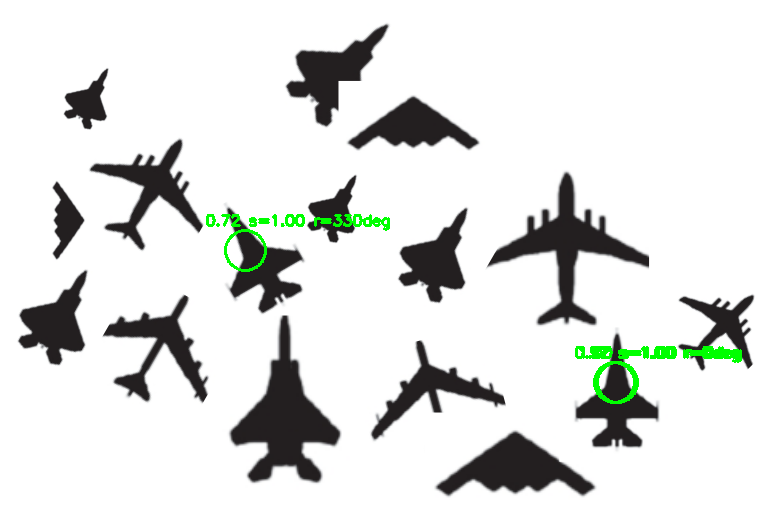
\includegraphics[width=0.6\textwidth]{pictures/chapter2/c02_p03_template_1_result.png}
                    \caption{Kết quả tìm kiếm máy bay trong hình với Template 1}
                \end{figure}
                \item Với template 2:
                \begin{figure}[H][H]
                    \centering
                    
\includegraphics[width=0.3\textwidth]{pictures/chapter2/c02_p04_template_2.png}
                    \caption{Template 2}
                \end{figure}
                Ta chọn các thông số như sau:
                \begin{lstlisting}
CANNY_LOW, CANNY_HIGH = 40, 120
ANGLE_BIN = 8               
ACC_REL_THRESH = 0.3        
MAX_PEAKS = 7             

# rotation & scale search space
ROT_STEP = 7               
SCALE_MIN, SCALE_MAX = 0.5, 1.5
SCALE_STEPS = 7             
                \end{lstlisting}
                \begin{figure}[H]
                    \centering
                    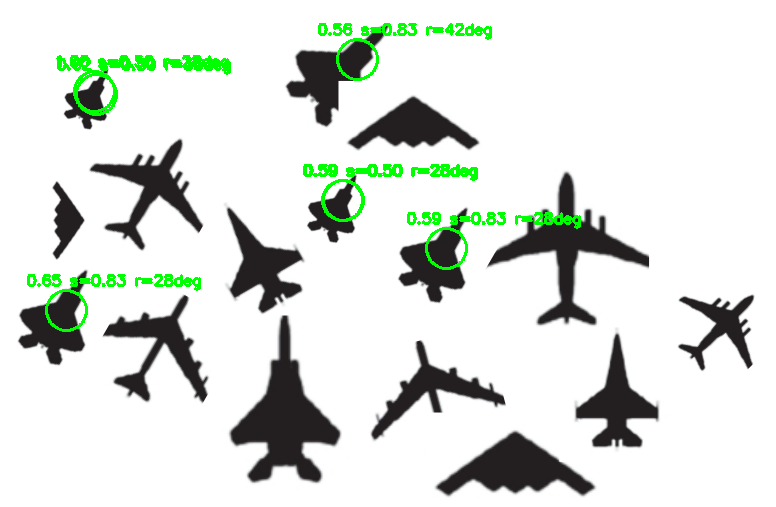
\includegraphics[width=0.6\textwidth]{pictures/chapter2/c02_p05_template_2_result.png}
                    \caption{Kết quả tìm kiếm máy bay trong hình với Template 2}
                \end{figure}
                \item Với template 3:
                \begin{figure}[H]
                    \centering
                    
\includegraphics[width=0.3\textwidth]{pictures/chapter2/c02_p06_template_3.png}
                    \caption{Template 3}
                \end{figure}
                Ta chọn các thông số như sau:
                \begin{lstlisting}
CANNY_LOW, CANNY_HIGH = 40, 120
ANGLE_BIN = 8               
ACC_REL_THRESH = 0.3        
MAX_PEAKS = 3             

# rotation & scale search space
ROT_STEP = 5               
SCALE_MIN, SCALE_MAX = 0.5, 1.5
SCALE_STEPS = 5            
                \end{lstlisting}
                \begin{figure}[H]
                    \centering
                    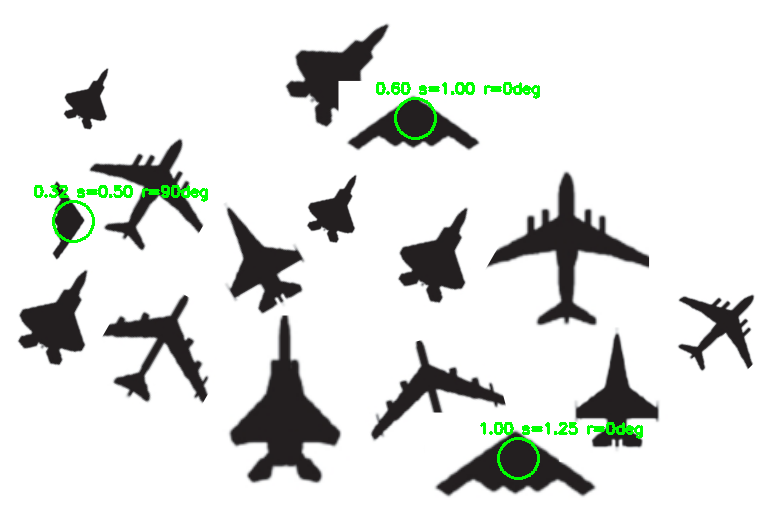
\includegraphics[width=0.6\textwidth]{pictures/chapter2/c02_p07_template_3_result.png}
                    \caption{Kết quả tìm kiếm máy bay trong hình với Template 3}
                \end{figure}
                \item Với template 4:
                \begin{figure}[H]
                    \centering
                    
\includegraphics[width=0.3\textwidth]{pictures/chapter2/c02_p08_template_4.png}
                    \caption{Template 4}
                \end{figure}
                Ta chọn các thông số như sau:
                \begin{lstlisting}
CANNY_LOW, CANNY_HIGH = 40, 120
ANGLE_BIN = 8               
ACC_REL_THRESH = 0.2        
MAX_PEAKS = 3            

# rotation & scale search space
ROT_STEP = 5             
SCALE_MIN, SCALE_MAX = 0.5, 1.5
SCALE_STEPS = 6              
       
                \end{lstlisting}
                \begin{figure}[H]
                    \centering
                    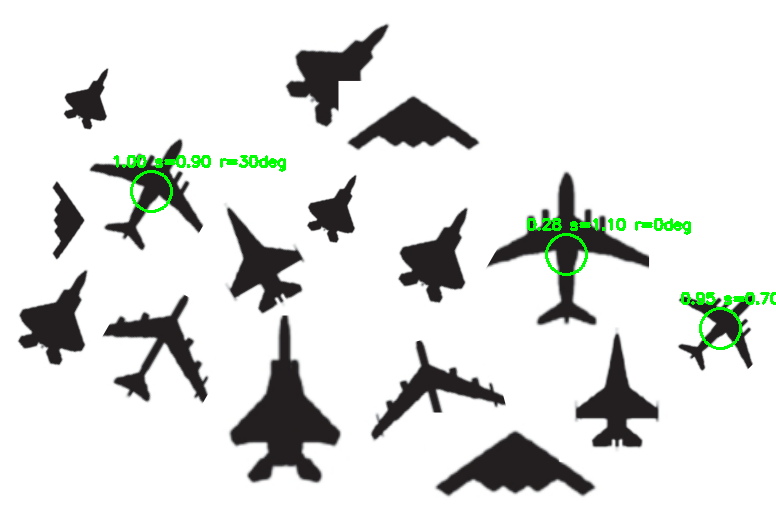
\includegraphics[width=0.6\textwidth]{pictures/chapter2/c02_p09_template_4_result.png}
                    \caption{Kết quả tìm kiếm máy bay trong hình với Template 4}
                \end{figure}
                \item Với template 5:
                \begin{figure}[H]
                    \centering
                    
\includegraphics[width=0.3\textwidth]{pictures/chapter2/c02_p10_template_5.png}
                    \caption{Template 5}
                \end{figure}
                Ta chọn các thông số như sau:
                \begin{lstlisting}
CANNY_LOW, CANNY_HIGH = 40, 120
ANGLE_BIN = 8               
ACC_REL_THRESH = 0.3        
MAX_PEAKS = 2             

# rotation & scale search space
ROT_STEP = 5               
SCALE_MIN, SCALE_MAX = 0.5, 1.5
SCALE_STEPS = 5             
                \end{lstlisting}
                \begin{figure}[H]
                    \centering
                    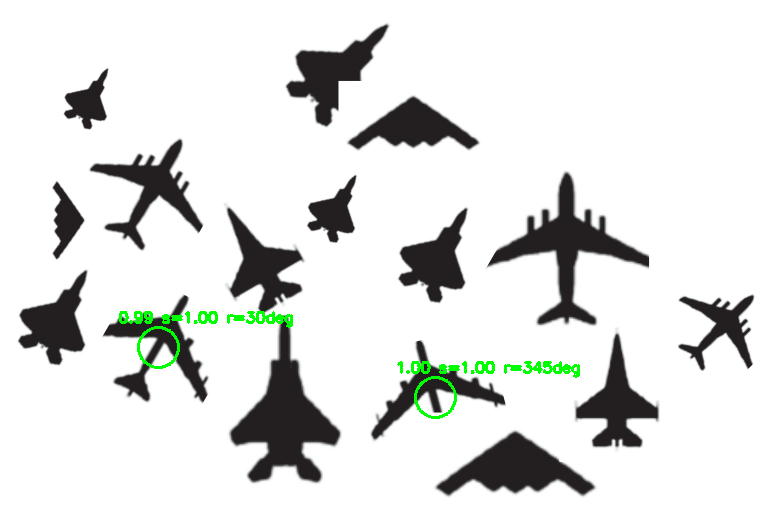
\includegraphics[width=0.6\textwidth]{pictures/chapter2/c02_p11_template_5_result.png}
                    \caption{Kết quả tìm kiếm máy bay trong hình với Template 5}
                \end{figure}
                \item Với template 6:
                \begin{figure}[H]
                    \centering
                    
\includegraphics[width=0.3\textwidth]{pictures/chapter2/c02_p12_template_6.png}
                    \caption{Template 6}
                \end{figure}
                Ta chọn các thông số như sau:
                \begin{lstlisting}
CANNY_LOW, CANNY_HIGH = 40, 120
ANGLE_BIN = 8               
ACC_REL_THRESH = 0.3        
MAX_PEAKS = 1             

# rotation & scale search space
ROT_STEP = 5               
SCALE_MIN, SCALE_MAX = 0.5, 1.5
SCALE_STEPS = 5             
                \end{lstlisting}
                \begin{figure}[H]
                    \centering
                    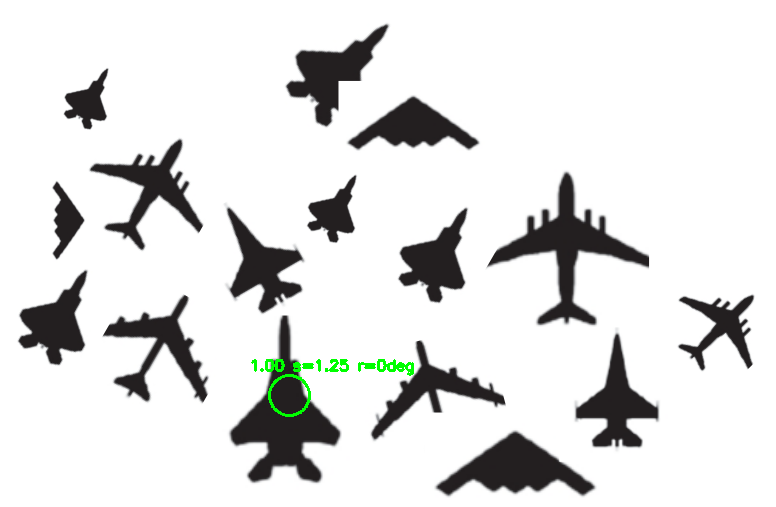
\includegraphics[width=0.6\textwidth]{pictures/chapter2/c02_p13_template_6_result.png}
                    \caption{Kết quả tìm kiếm máy bay trong hình với Template 6}
                \end{figure}
            \end{itemize}
    \subsection{Tìm vị trí các máy bay trong hình bằng phương pháp genral hough transform của OpenCV}
        \subsubsection{Các bước thực hiện}
            \begin{itemize}
                \item Tạo template các máy bay trong hình và load template cùng scene như trên:
                \item Detect edges và khởi tạo Ballard:
                \begin{lstlisting}
scene_edges = cv2.Canny(scene_gray, CANNY_LOW, CANNY_HIGH)

# Create Ballard
ght = cv2.createGeneralizedHoughBallard()
ght.setCannyLowThresh(CANNY_LOW)
ght.setCannyHighThresh(CANNY_HIGH)
ght.setMinDist(MIN_DIST)
ght.setVotesThreshold(VOTE_THRESH)
                \end{lstlisting}
                \item Khởi tạo GHT Ballard và vòng lặp tìm kiếm. Ballard không tự xoay/scale → ta tạo nhiều phiên bản template (xoay + scale), truyền từng cái vào Ballard (setTemplate) rồi gọi detect.
                \begin{lstlisting}
for scale in SCALES:
        for angle in ROTATIONS:

            # generate transformed template
            tpl_rs = rotate_and_scale(tpl0, angle, scale)
            th, tw = tpl_rs.shape[:2]
            if th < 5 or tw < 5: 
                continue
            if th >= Hs or tw >= Ws:
                continue

            tpl_edges = cv2.Canny(tpl_rs, CANNY_LOW, CANNY_HIGH)

            # Set template for Ballard
            ght.setTemplate(tpl_edges)

            # Detect, returns (positions, votes)
            pos, votes = ght.detect(scene_edges)

            if pos is None or len(pos) == 0:
                continue

            pos = np.array(pos).reshape(-1, 2)  # Ballard returns only (x,y)
            votes = np.array(votes).reshape(-1)

            for (x, y), v in zip(pos, votes):
                detections.append({
                    "x": int(x - tw//2),
                    "y": int(y - th//2),
                    "w": tw,
                    "h": th,
                    "vote": int(v),
                    "scale": float(scale),
                    "angle": float(angle)
                })
                \end{lstlisting}
                \item Lọc và hiển thị kết quả:
                \begin{lstlisting}
filtered = nms(detections, thresh=0.3)
vis = scene_color.copy()
    for d in filtered:
        x, y, w, h = d["x"], d["y"], d["w"], d["h"]
        cv2.rectangle(vis, (x, y), (x+w, y+h), (0,255,0), 2)
        cv2.putText(vis,
                    f"v={d['vote']} s={d['scale']:.2f} a={d['angle']}",
                    (x, max(0,y-10)),
                    cv2.FONT_HERSHEY_SIMPLEX, 0.5,
                    (0,255,0), 2)
cv2.imwrite(OUT_PATH, vis)
print("Saved result to:", OUT_PATH)

try:
    cv2.imshow("GHT Ballard", vis)
    cv2.waitKey(0)
except:
    pass
                \end{lstlisting}
            \end{itemize}
        \subsubsection{Kết quả thu được}
            \begin{itemize}
                \item Với template 1:
                \hspace*{0.6cm}Ta chọn các thông số như sau:
                \begin{lstlisting}
ANGLE_STEP = 5
SCALE_MIN, SCALE_MAX = 0.6, 1.4
SCALE_STEPS = 9
CANNY_LOW = 40
CANNY_HIGH = 120
MIN_DIST = 20
VOTE_THRESH = 200  
MAX_FINAL = 2
                \end{lstlisting}
                \begin{figure}[H]
                    \centering
                    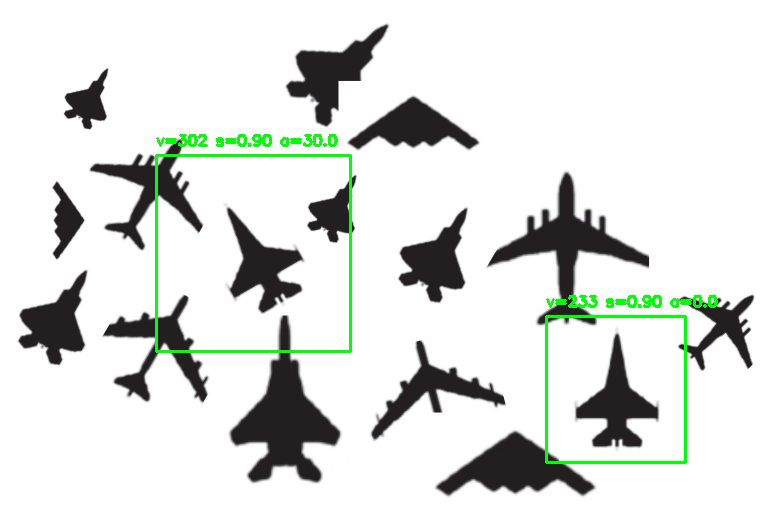
\includegraphics[width=0.6\textwidth]{pictures/chapter2/c02_p14_template_1_result_OCV.png}
                    \caption{Kết quả tìm kiếm máy bay trong hình với Template 1 bằng OpenCV GHT Ballard}
                \end{figure}
                \item Với template 2:
                \hspace*{0.6cm}Ta chọn các thông số như sau:
                \begin{lstlisting}
ANGLE_STEP = 4
SCALE_MIN, SCALE_MAX = 0.5, 1.5
SCALE_STEPS = 6
CANNY_LOW = 40
CANNY_HIGH = 120
MIN_DIST = 40
VOTE_THRESH = 80
MAX_FINAL = 7
                \end{lstlisting}
                \begin{figure}[H]
                    \centering
                    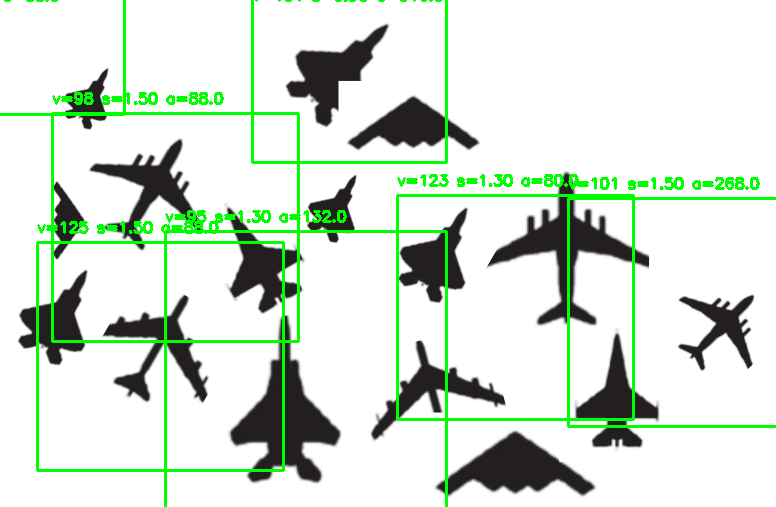
\includegraphics[width=0.6\textwidth]{pictures/chapter2/c02_p15_template_2_result_OCV.png}
                    \caption{Kết quả tìm kiếm máy bay trong hình với Template 2 bằng OpenCV GHT Ballard}
                \end{figure}
                \item Với template 3:
                \hspace*{0.6cm}Ta chọn các thông số như sau:
                \begin{lstlisting}
ANGLE_STEP = 6
SCALE_MIN, SCALE_MAX = 0.5, 1.25
SCALE_STEPS = 14
CANNY_LOW = 40
CANNY_HIGH = 120
MIN_DIST = 50
VOTE_THRESH = 90
MAX_FINAL = 3
                \end{lstlisting}
                \begin{figure}[H]
                    \centering
                    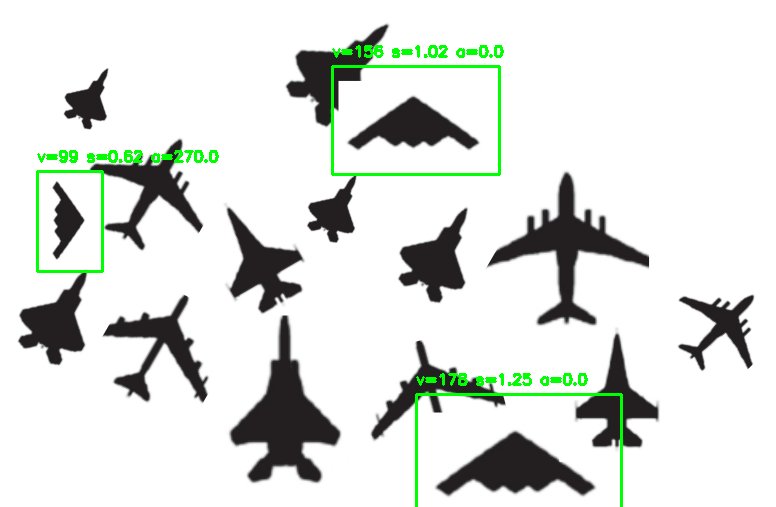
\includegraphics[width=0.6\textwidth]{pictures/chapter2/c02_p16_template_3_result_OCV.png}
                    \caption{Kết quả tìm kiếm máy bay trong hình với Template 3 bằng OpenCV GHT Ballard}
                \end{figure}
                \item Với template 4:
                \hspace*{0.6cm}Ta chọn các thông số như sau:
                \begin{lstlisting}
ANGLE_STEP = 4
SCALE_MIN, SCALE_MAX = 0.5, 1.5
SCALE_STEPS = 6
CANNY_LOW = 40
CANNY_HIGH = 120
MIN_DIST = 40
VOTE_THRESH = 80
MAX_FINAL = 3
                \end{lstlisting}
                \begin{figure}[H]
                    \centering
                    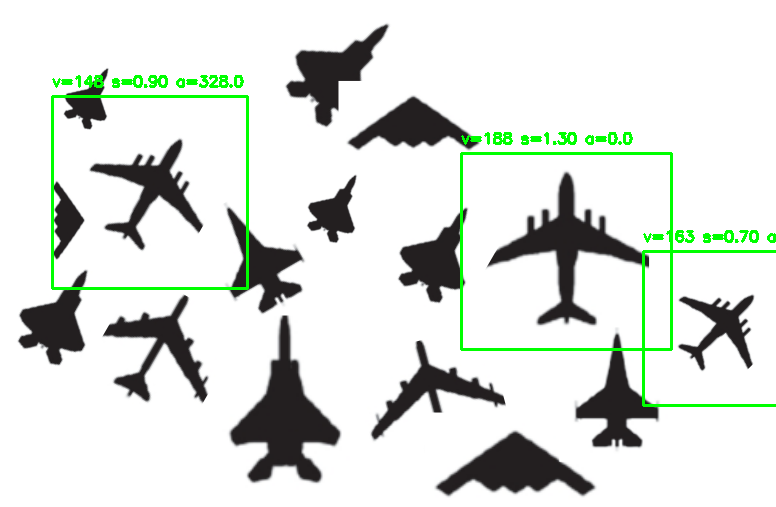
\includegraphics[width=0.6\textwidth]{pictures/chapter2/c02_p17_template_4_result_OCV.png}
                    \caption{Kết quả tìm kiếm máy bay trong hình với Template 4 bằng OpenCV GHT Ballard}       
                \end{figure}
                \item Với template 5:
                \hspace*{0.6cm}Ta chọn các thông số như sau:
                \begin{lstlisting}
ANGLE_STEP = 5
SCALE_MIN, SCALE_MAX = 0.5, 1.5
SCALE_STEPS = 7
CANNY_LOW = 40
CANNY_HIGH = 120
MIN_DIST = 40
VOTE_THRESH = 80
MAX_FINAL = 2
                \end{lstlisting}
                \begin{figure}[H]
                    \centering
                    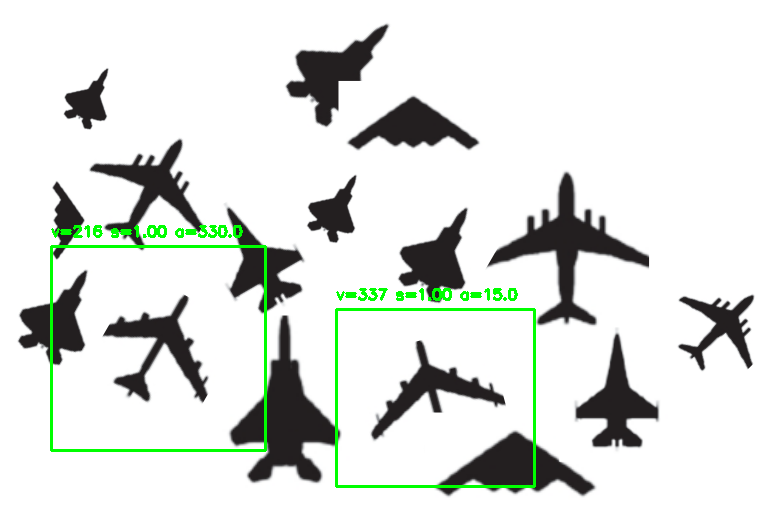
\includegraphics[width=0.6\textwidth]{pictures/chapter2/c02_p18_template_5_result_OCV.png}
                    \caption{Kết quả tìm kiếm máy bay trong hình với Template 5 bằng OpenCV GHT Ballard}       
                \end{figure}
                \item Với template 6:
                \hspace*{0.6cm}Ta chọn các thông số như sau:
                \begin{lstlisting}
ANGLE_STEP = 5
SCALE_MIN, SCALE_MAX = 0.5, 1.5
SCALE_STEPS = 7
CANNY_LOW = 40
CANNY_HIGH = 120
MIN_DIST = 40
VOTE_THRESH = 80
MAX_FINAL = 1
                \end{lstlisting}
                \begin{figure}[H]
                    \centering
                    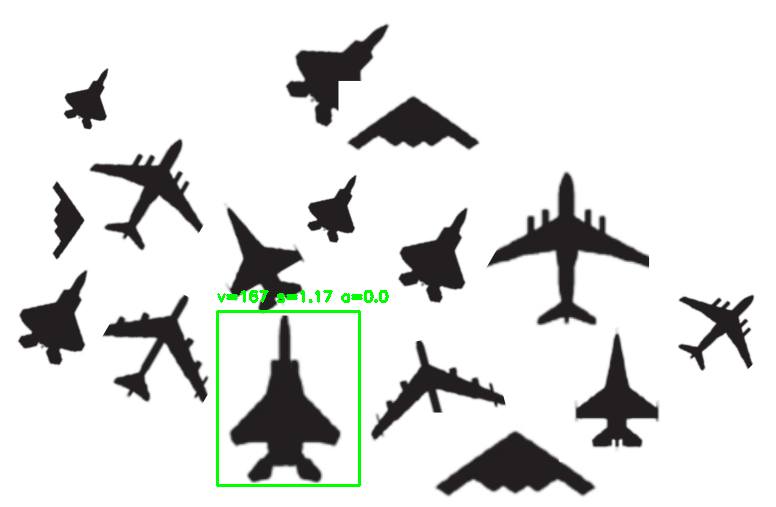
\includegraphics[width=0.6\textwidth]{pictures/chapter2/c02_p19_template_6_result_OCV.png}
                    \caption{Kết quả tìm kiếm máy bay trong hình với Template 6 bằng OpenCV GHT Ballard}       
                \end{figure}
                \end{itemize}
    \subsection{Nhận xét}
        \begin{itemize}
            \item Kết quả thu được từ cả hai phương pháp GHT tự lập trình và GHT OpenCV đều khá tốt, có thể phát hiện được hầu hết các máy bay trong hình với các template khác nhau.
            \item Cả 2 phuơng pháp đều cần lập trình thêm phần xoay và scale cho template để có thể tìm kiếm đa dạng các đối tượng trong hình cùng với việc lọc kết quả bằng NMS để giữ lại các đỉnh tốt nhất. 
            \item GHT OpenCV cung cấp một giải pháp nhanh chóng và tiện lợi, tuy nhiên việc thiếu khả năng tùy chỉnh sâu có thể hạn chế hiệu suất trong một số trường hợp cụ thể, ví dụ đối với truờng hợp template số 2, GHT OpenCV xử lý chưa đuợc tốt do không thể can thiệp quá sâu vào bên trong thuật toán.
            \item GHT tự lập trình cho phép kiểm soát chi tiết hơn về quá trình, linh động trong việc điều chỉnh các tham số và tối ưu hóa thuật toán cho các trường hợp cụ thể. Tuy nhiên, việc này đòi hỏi nhiều thời gian và công sức để phát triển và tinh chỉnh.
            \item Cả hai phương pháp đều yêu cầu lựa chọn tham số cẩn thận (như ngưỡng Canny, bước góc, phạm vi tỉ lệ) để đạt được kết quả tốt nhất.
        \end{itemize}


            
            
            